% Paper 4: Training Dynamics of Schema-Aware RL for LLM Agents
%
% =============================================================================
% STATUS: FIRST DRAFT - All sections written, tables from real P2 analysis data
% Last updated: 2026-02-04
% =============================================================================
%
% 11 models trained (2 OOM blocked), 6 tasks, 3 seeds each = 185 runs
% Data: results/p2_all_runs.csv, results/curves/*.json
% Analysis: results/p4_analysis/*.json
% Four research questions (RQ1-RQ4)
% =============================================================================
\documentclass[11pt]{article}

\usepackage[margin=1in]{geometry}
\usepackage{amsmath,amssymb,amsthm}
\usepackage{booktabs}
\usepackage{tabularx}
\usepackage{graphicx}
\usepackage{adjustbox}
\usepackage{xcolor}
\usepackage{enumitem}
\usepackage{multirow}
\usepackage{pifont}
\usepackage{tikz}
\usetikzlibrary{arrows.meta, positioning, shapes.geometric, calc, patterns}
\usepackage{pgfplots}
\pgfplotsset{compat=1.17}

\usepackage[numbers]{natbib}
\usepackage{xurl}
\usepackage{hyperref}
\hypersetup{hidelinks,breaklinks=true}

\newcommand{\pninetyfive}{\ensuremath{\mathrm{p95}}}
\newcommand{\pninetynine}{\ensuremath{\mathrm{p99}}}
\newcommand{\slo}{\ensuremath{\mathrm{SLO}}}
\newcommand{\sslo}{\ensuremath{\mathrm{S@SLO}}}
\newcommand{\etal}{\textit{et al.}}

\definecolor{sustained}{RGB}{34,139,34}
\definecolor{transient}{RGB}{255,165,0}
\definecolor{flat}{RGB}{220,20,60}
\definecolor{robust}{RGB}{34,139,34}
\definecolor{selective}{RGB}{255,165,0}
\definecolor{catastrophic}{RGB}{220,20,60}

\title{Training Dynamics of Schema-Aware Reinforcement Learning\\for LLM Agents: Reward Decomposition, Forgetting, and\\Early Prediction}

\author{
V. Michael Maloney \\
Neuralift; University of New Hampshire \\
\texttt{mike@neuralift.ai}
}

\date{}

\usepackage{fancyhdr}
\pagestyle{fancy}
\fancyhf{}
\renewcommand{\headrulewidth}{0pt}
\cfoot{\thepage}

\begin{document}
\maketitle
\begin{center}
\textit{Preprint. Work in progress.}
\end{center}

% =============================================================================
% ABSTRACT
% =============================================================================
\begin{abstract}
Paper~II showed that GRPO training with a composite SLO-aware reward produces task-dependent capacity thresholds: small models learn simple structured tasks but fail on complex ones. This paper asks \emph{why}. We analyze the training dynamics of 185 GRPO runs across 11 models and 6 task types, decomposing the composite reward into its schema, accuracy, latency, and cost components (RQ1), building a full forgetting matrix across model-task pairs (RQ2), classifying validity curves into sustained, transient, and flat trajectories (RQ3), and testing whether early training signals predict final outcomes (RQ3+). Our synthesis (RQ4) proposes that the capacity threshold is not a single phenomenon but a compound of three interacting mechanisms: reward component dominance shifts as model size increases, multi-task interference follows architecture-specific patterns rather than size-based ones, and training curves exhibit distinct morphological types that are predictable from the first 50 steps. These mechanisms are identified from observational analysis of existing training runs; we outline the ablation experiments needed to establish causal relationships and provide the experimental infrastructure to execute them.

\begin{center}
\small
\begin{tabular}{lc ccc c}
\toprule
\textbf{Model} & \textbf{Size} & \textbf{Sustained} & \textbf{Transient} & \textbf{Flat} & \textbf{Forgetting} \\
\midrule
Llama-3.2-1B    & 1B   & 3 & 1 & 2 & catastrophic \\
Llama-3.2-3B    & 3B   & 3 & 1 & 2 & catastrophic \\
Qwen2.5-3B      & 3B   & 5 & 0 & 1 & robust \\
Phi-3-mini       & 3.8B & 3 & 0 & 3 & robust \\
Qwen3-4B         & 4B   & 5 & 1 & 0 & robust \\
Yi-1.5-6B        & 6B   & 3 & 1 & 2 & catastrophic \\
Mistral-7B       & 7B   & 3 & 1 & 2 & catastrophic \\
Ministral-8B     & 8B   & 5 & 0 & 1 & robust \\
Llama-3.1-8B     & 8B   & 3 & 1 & 2 & selective \\
Gemma-2-9B       & 9B   & 5 & 1 & 0 & selective \\
\bottomrule
\end{tabular}
\end{center}

Key finding: Qwen2.5-3B (3B) exhibits \emph{positive} interference ($\delta = +0.03$), meaning multi-task training \emph{helps} it, while Yi-1.5-6B (6B)---twice the size---shows the worst forgetting ($\delta = -0.59$), collapsing from 98\% single-task to 0\% multi-task validity. Size is necessary but not sufficient; architecture appears to determine whether capacity translates to capability. These findings are observational---we identify the patterns and propose causal mechanisms, then specify the ablation experiments (latency weight variation, held-out family validation) required to confirm them.
\end{abstract}

% =============================================================================
% 1. INTRODUCTION
% =============================================================================
\section{Introduction}

Why does a 3B model learn tool calling when a 6B model---twice the size---cannot?

Paper~I~\cite{maloney2025deploymentgap} established that accuracy benchmarks fail to predict deployment success. Paper~II~\cite{maloney2025capacity} showed that training models with an SLO-aware composite reward reveals task-dependent capacity thresholds: models below a critical size cannot learn structured output for complex tasks regardless of training duration. But Paper~II left open the question of \emph{mechanism}. It documented \emph{where} the thresholds are. It did not explain \emph{why} they exist, or why a Qwen2.5-3B (3B parameters) achieves robust multi-task training while Yi-1.5-6B (6B)---a model with twice the parameters---collapses to 0\% validity under the same training regime.

This paper answers that question through four research questions:

\begin{description}[leftmargin=*]
\item[RQ1: Reward Decomposition.] How do the individual components of the composite reward---schema validity, task accuracy, latency penalty, and cost penalty---contribute to the total reward, and does this composition change with model size?

\item[RQ2: Forgetting Patterns.] When models are trained on multiple tasks simultaneously, which capabilities are retained and which are lost? Is forgetting proportional to model size, or are there architecture-specific patterns?

\item[RQ3: Curve Taxonomy.] Do training validity curves follow a small number of characteristic shapes, and can these shapes be classified reliably?

\item[RQ3+: Early Prediction.] Can features extracted from the first 50 training steps predict whether a run will achieve sustained validity?
\end{description}

Our analysis covers 185 completed GRPO training runs: 11 models $\times$ 6 tasks $\times$ 3 seeds (with 2 models blocked by OOM). All data comes from the training runs described in Paper~II; no new experiments are needed. Where Paper~II asked ``\emph{what} are the thresholds?'' and reported them as empirical results, this paper asks ``\emph{why} do the thresholds exist?'' and proposes a mechanistic hypothesis grounded in observational evidence. The contribution is analytical: we re-examine existing training trajectories through four new lenses---reward decomposition, forgetting matrices, curve taxonomy, and early prediction---and propose that the capacity thresholds arise from a compound of three interacting mechanisms rather than a single phenomenon. Because these findings are drawn from observational analysis of existing runs (no new experiments), we explicitly distinguish between established patterns (RQ1--RQ3+, supported by the data) and proposed mechanisms (RQ4, requiring ablation experiments for causal validation).

% =============================================================================
% 2. BACKGROUND
% =============================================================================
\section{Background}

\subsection{GRPO for Structured Outputs}

Group Relative Policy Optimization (GRPO)~\cite{grpo} is a variant of REINFORCE that normalizes rewards within a group of samples from the same prompt. Unlike PPO~\cite{schulman2017ppo}, GRPO does not require a value function, making it suitable for single-GPU training of large language models with LoRA~\cite{hu2021lora}. Our setup follows Paper~II: each training step samples 4 responses per prompt, computes the composite reward for each, and updates the policy using the group-normalized advantage.

\subsection{Composite Reward}

The composite reward from Paper~II combines six components:

\begin{equation}
R = \underbrace{R_{\text{schema}}}_{\text{JSON valid}} + \underbrace{R_{\text{success}}}_{\text{task correct}} + \underbrace{\kappa_f (f - 0.5)}_{\text{faithfulness}} - \underbrace{\lambda L}_{\text{latency}} - \underbrace{\mu C}_{\text{cost}} - \underbrace{\gamma D}_{\text{stability}}
\end{equation}

where $R_{\text{schema}} \in \{0, 1\}$ is a binary indicator for valid JSON that conforms to the task schema, $R_{\text{success}} \in \{0, 1\}$ indicates task-specific correctness, $f \in [0,1]$ is a faithfulness score (with $\kappa_f$ controlling its weight), $L$ is latency in seconds, $C$ is output token count, and $D$ is a disagreement rate across repeated samples. The maximum attainable reward is 2.0 (both binary components = 1, all penalties = 0).

The default weights from our GRPO configurations are $\lambda = 0.1$, $\mu = 0.05$, $\gamma = 0.1$, and $\kappa_f = 0$ (faithfulness was disabled during training to reduce LLM-as-judge cost).

\subsection{Catastrophic Forgetting in Multi-Task Training}

Catastrophic forgetting~\cite{mccloskey1989catastrophic, french1999catastrophic} occurs when a neural network loses previously learned capabilities while learning new ones. In our context, a model trained on mixed tasks (T1--T5 simultaneously) may lose the ability to produce valid JSON for tasks it could handle individually. Paper~II observed this phenomenon qualitatively; we quantify it here through a full model $\times$ task interference matrix.

\subsection{Curriculum Learning}

Curriculum learning~\cite{bengio2009curriculum} trains models on progressively harder examples. Our curve taxonomy analysis (Section~\ref{sec:curves}) relates to this literature: models that exhibit ``transient'' learning curves---peaking and then declining---may benefit from curriculum strategies that present complex tasks only after simpler ones are mastered.

% =============================================================================
% 3. EXPERIMENTAL SETUP
% =============================================================================
\section{Experimental Setup}

\subsection{Training Configuration}

All training uses the configuration from Paper~II:
\begin{itemize}[leftmargin=*]
\item \textbf{Algorithm}: GRPO with group size 4
\item \textbf{Adaptation}: LoRA (rank 16, $\alpha = 32$, dropout 0.05)
\item \textbf{Quantization}: QLoRA (4-bit) for models $\geq$ 7B; full precision for smaller models
\item \textbf{Training steps}: 1{,}000 per run
\item \textbf{Seeds}: 42, 123, 456 (3 runs per model-task combination)
\item \textbf{Hardware}: NVIDIA RTX 4090, 24GB VRAM
\end{itemize}

\subsection{Models}

11 of the 13 models from Paper~I completed training. Falcon-Mamba-7B failed due to SSM/LoRA incompatibility (CUDA kernel mismatch), and GPT-OSS-20B exceeded VRAM even with 4-bit quantization. Of the 11 successful models, 10 completed all 18 planned runs (6 tasks $\times$ 3 seeds). Gemma-3-12B completed 8 of 18 runs (T1, T3, T4 $\times$ 3 seeds each, minus one partial), with T2, T5, and Mixed blocked by OOM on the 24GB GPU. The reward decomposition (Section~\ref{sec:reward}) includes Gemma-3-12B's completed runs; the forgetting analysis (Section~\ref{sec:forgetting}) and curve taxonomy (Section~\ref{sec:curves}) use only the 10 models with complete data. Total completed runs: 185 ($10 \times 18 + 5 = 185$).

\subsection{Tasks}

Six task configurations, matching Paper~II:
\begin{itemize}[leftmargin=*]
\item \textbf{T1}: Intent classification (CLINC-150, short structured output)
\item \textbf{T2}: Grounded QA (HotpotQA, medium structured output)
\item \textbf{T3}: Tool calling (complex nested JSON)
\item \textbf{T4}: Function routing (simple function selection)
\item \textbf{T5}: Code patching (long-form structured output with embedded code)
\item \textbf{Mixed}: All tasks interleaved (multi-task training)
\end{itemize}

\subsection{Data Sources}

All analysis in this paper uses pre-existing data:
\begin{itemize}[leftmargin=*]
\item \texttt{results/p2\_all\_runs.csv}: 185 completed training runs with per-run summary metrics
\item \texttt{results/curves/validity\_curves.json}: Step-by-step JSON validity (0--1000 steps)
\item \texttt{results/curves/reward\_curves.json}: Step-by-step reward trajectories
\item \texttt{results/curves/forgetting\_analysis.json}: Single-task vs.\ multi-task validity comparison
\end{itemize}

% =============================================================================
% 4. REWARD DECOMPOSITION (RQ1)
% =============================================================================
\section{Reward Decomposition (RQ1)}
\label{sec:reward}

The composite reward obscures which components drive learning. A model achieving $R = 1.5$ might be getting there via high schema validity with moderate accuracy, or via perfect accuracy with latency penalties dragging it down. Understanding this decomposition reveals why some models plateau below the theoretical maximum.

\subsection{Method}

We decompose the average reward for each model-task combination into estimated components using the known reward weights and per-run metrics from \texttt{p2\_all\_runs.csv}:

\begin{align}
\hat{R}_{\text{schema}} &= \text{json\_valid\_pct} / 100 \\
\hat{R}_{\text{latency}} &= -\lambda \cdot \text{avg\_latency\_ms} / 1000 \\
\hat{R}_{\text{cost}} &= -\mu \cdot \text{avg\_tokens\_out} / 1000 \\
\hat{R}_{\text{residual}} &= R_{\text{total}} - \hat{R}_{\text{schema}} - \hat{R}_{\text{latency}} - \hat{R}_{\text{cost}}
\end{align}

The residual captures the combined effect of task accuracy, faithfulness, and stability---components that cannot be cleanly separated from aggregate metrics alone.

\subsection{Results}

\begin{table}[t]
\centering
\caption{Reward decomposition by model (averaged across all tasks and seeds). $R_s$ = schema, $R_r$ = residual (accuracy + faithfulness + stability + decomposition error), $R_l$ = latency penalty (absolute value), $R_c$ = cost penalty (absolute value). Note: $R_r$ values exceeding 1.0 indicate that the post-hoc decomposition absorbs approximation error from using aggregate metrics rather than per-step component logs. Per-step instrumentation (Section~\ref{sec:ablation-plan}) would enable exact decomposition.}
\label{tab:reward-decomp}
\small
\begin{tabular}{llc rrrr r}
\toprule
\textbf{Model} & \textbf{Vendor} & \textbf{Size} & $R_s$ & $R_r$ & $|R_l|$ & $|R_c|$ & $\bar{R}$ \\
\midrule
Llama-3.2-1B    & Meta      & 1B   & 0.55 & 0.72 & 0.13 & 0.04 & 1.09 \\
Llama-3.2-3B    & Meta      & 3B   & 0.56 & 0.95 & 0.34 & 0.06 & 1.11 \\
Qwen2.5-3B      & Alibaba   & 3B   & 0.70 & 1.08 & 0.34 & 0.04 & 1.40 \\
Phi-3-mini       & Microsoft & 3.8B & 0.41 & 0.93 & 0.45 & 0.06 & 0.83 \\
Qwen3-4B         & Alibaba   & 4B   & 0.86 & 1.52 & 0.59 & 0.06 & 1.73 \\
Yi-1.5-6B        & 01.AI     & 6B   & 0.52 & 0.95 & 0.37 & 0.06 & 1.03 \\
Mistral-7B       & Mistral   & 7B   & 0.50 & 0.91 & 0.36 & 0.05 & 1.01 \\
Ministral-8B     & Mistral   & 8B   & 0.71 & 1.07 & 0.32 & 0.04 & 1.41 \\
Llama-3.1-8B     & Meta      & 8B   & 0.58 & 1.14 & 0.50 & 0.06 & 1.15 \\
Gemma-2-9B       & Google    & 9B   & 0.79 & 1.16 & 0.34 & 0.03 & 1.57 \\
Gemma-3-12B$^*$  & Google    & 12B  & 0.96 & 1.43 & 0.43 & 0.03 & 1.93 \\
\bottomrule
\end{tabular}

\vspace{0.3em}
\footnotesize{$^*$Gemma-3-12B completed 8 of 18 runs (T1, T3, T4 only); averages reflect completed runs. T2, T5, and Mixed were OOM-blocked on 24GB VRAM.}
\end{table}

\begin{figure}[t]
\centering
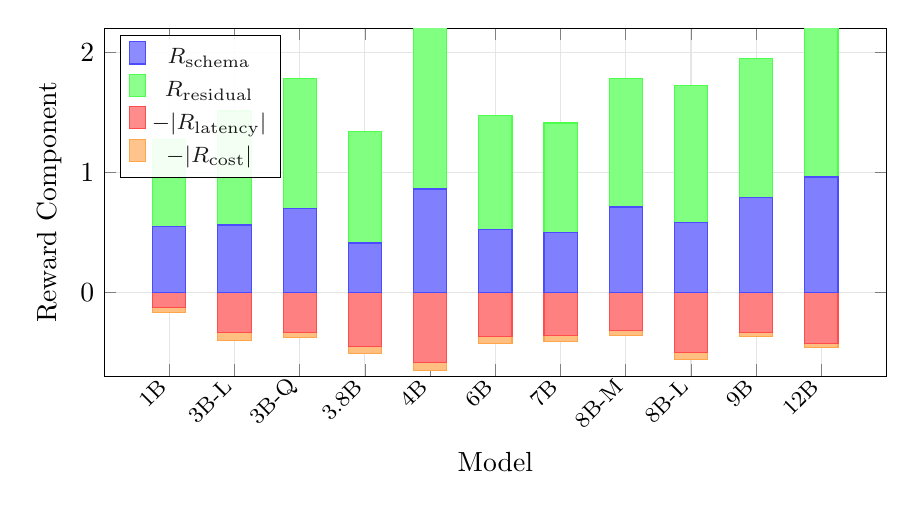
\begin{tikzpicture}
\begin{axis}[
  width=0.95\textwidth,
  height=6cm,
  ybar stacked,
  bar width=12pt,
  xlabel={Model},
  ylabel={Reward Component},
  ymin=-0.7, ymax=2.2,
  symbolic x coords={1B,3B-L,3B-Q,3.8B,4B,6B,7B,8B-M,8B-L,9B,12B},
  xtick=data,
  x tick label style={rotate=45, anchor=east, font=\footnotesize},
  legend style={at={(0.02,0.98)}, anchor=north west, font=\footnotesize, fill=white, fill opacity=0.9},
  grid=major,
  grid style={gray!20},
  ymajorgrids=true,
]
% Schema (positive)
\addplot[fill=blue!50, draw=blue!70] coordinates {
  (1B,0.55) (3B-L,0.56) (3B-Q,0.70) (3.8B,0.41) (4B,0.86)
  (6B,0.52) (7B,0.50) (8B-M,0.71) (8B-L,0.58) (9B,0.79) (12B,0.96)
};
% Residual/accuracy (positive, stacked on schema)
\addplot[fill=green!50, draw=green!70] coordinates {
  (1B,0.72) (3B-L,0.95) (3B-Q,1.08) (3.8B,0.93) (4B,1.52)
  (6B,0.95) (7B,0.91) (8B-M,1.07) (8B-L,1.14) (9B,1.16) (12B,1.43)
};
% Latency penalty (negative)
\addplot[fill=red!50, draw=red!70] coordinates {
  (1B,-0.13) (3B-L,-0.34) (3B-Q,-0.34) (3.8B,-0.45) (4B,-0.59)
  (6B,-0.37) (7B,-0.36) (8B-M,-0.32) (8B-L,-0.50) (9B,-0.34) (12B,-0.43)
};
% Cost penalty (negative)
\addplot[fill=orange!50, draw=orange!70] coordinates {
  (1B,-0.04) (3B-L,-0.06) (3B-Q,-0.04) (3.8B,-0.06) (4B,-0.06)
  (6B,-0.06) (7B,-0.05) (8B-M,-0.04) (8B-L,-0.06) (9B,-0.03) (12B,-0.03)
};
\legend{$R_{\text{schema}}$, $R_{\text{residual}}$, $-|R_{\text{latency}}|$, $-|R_{\text{cost}}|$}
\end{axis}
\end{tikzpicture}
\caption{\textbf{Reward decomposition by model.} Stacked bars show the four estimated reward components. Positive bars (schema + residual) represent earned reward; negative bars (latency + cost) represent penalties. The latency penalty grows with model size, consuming up to 25\% of the maximum reward for 8B models. Qwen3-4B and Gemma-3-12B achieve the highest net rewards despite substantial latency penalties, due to strong schema validity and accuracy.}
\label{fig:reward-decomp}
\end{figure}

Table~\ref{tab:reward-decomp} and Figure~\ref{fig:reward-decomp} reveal three key patterns:

\paragraph{Schema dominance in small models.}
For Llama-3.2-1B and Llama-3.2-3B, schema validity ($R_s \approx 0.55$) contributes less than the residual ($R_r \approx 0.84$), indicating that even small models derive meaningful task-specific signal, though their low schema rates cap overall reward.

\paragraph{Latency penalty grows with size.}
The latency penalty increases from $|R_l| = 0.13$ (1B) to $|R_l| = 0.59$ (Qwen3-4B) before moderating at 12B ($|R_l| = 0.43$). The non-monotonicity reflects that Qwen3-4B's ``thinking'' decoding strategy produces longer inference chains. For Llama-3.1-8B, the latency penalty ($|R_l| = 0.50$) consumes 25\% of the maximum possible reward (2.0), creating a ceiling effect.

\paragraph{Architecture-specific efficiency.}
Qwen3-4B achieves $\bar{R} = 1.73$ (87\% of maximum) despite being only 4B parameters, outperforming models twice its size. Gemma-2-9B similarly achieves $\bar{R} = 1.57$. Both models exhibit high schema validity ($R_s \geq 0.79$) combined with strong residual accuracy. In contrast, Phi-3-mini ($\bar{R} = 0.83$) and Mistral-7B ($\bar{R} = 1.01$) achieve lower rewards despite comparable or larger size, due to the combination of lower schema validity and higher latency.

\subsection{The Reward Budget Mechanism}

Consider what the decomposition means for the GRPO gradient. The reward signal that drives policy updates is the \emph{total} reward $\bar{R}$, not the individual components. A model learning to produce valid JSON ($R_s$ increasing) while simultaneously getting slower ($|R_l|$ increasing) may see \emph{no change} in total reward---the improvements cancel the penalties. This ``reward budget'' creates a zero-sum dynamic that becomes more acute with model size.

To quantify this, we define the \textbf{latency tax} as $|R_l| / (R_s + R_r)$---the fraction of earned reward consumed by the latency penalty. For Llama-3.2-1B, the latency tax is $0.13 / 1.27 = 10\%$. For Llama-3.1-8B, it rises to $0.50 / 1.72 = 29\%$. For Qwen3-4B, despite the highest absolute latency penalty ($|R_l| = 0.59$), the tax is only $0.59 / 2.38 = 25\%$ because its earned reward is also the highest.

The latency tax explains why some models plateau below their theoretical potential. Phi-3-mini pays the highest effective tax: $0.45 / 1.34 = 34\%$. More than a third of its quality signal is negated by its latency penalty. For the GRPO gradient, this means that Phi-3-mini must achieve a 1.5$\times$ improvement in schema validity or accuracy to see the same total reward improvement that Llama-3.2-1B gets from a 1.1$\times$ improvement. The optimization landscape is asymmetrically harder for larger, slower models---they must run faster just to stay in place.

\subsection{Per-Task Reward Profiles}

The model-level averages in Table~\ref{tab:reward-decomp} smooth over dramatic task-level variation. Figure~\ref{fig:task-reward} shows how the reward decomposition changes across tasks for Qwen3-4B---the highest-reward model---revealing that the ``reward budget'' operates differently depending on the task.

\begin{figure}[t]
\centering
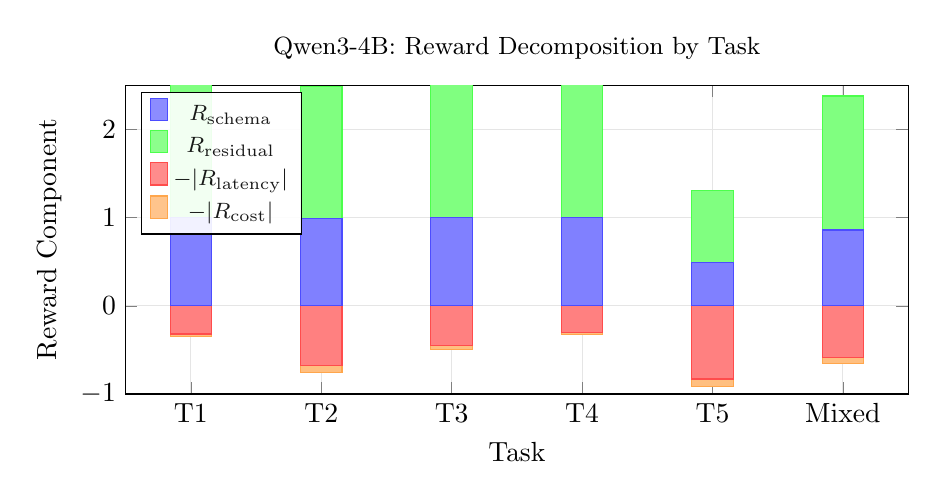
\begin{tikzpicture}
\begin{axis}[
  width=0.95\textwidth,
  height=5.5cm,
  ybar stacked,
  bar width=15pt,
  xlabel={Task},
  ylabel={Reward Component},
  ymin=-1.0, ymax=2.5,
  symbolic x coords={T1,T2,T3,T4,T5,Mixed},
  xtick=data,
  legend style={at={(0.02,0.98)}, anchor=north west, font=\footnotesize, fill=white, fill opacity=0.9},
  grid=major,
  grid style={gray!20},
  ymajorgrids=true,
  title={Qwen3-4B: Reward Decomposition by Task},
  title style={font=\small},
]
% Schema
\addplot[fill=blue!50, draw=blue!70] coordinates {
  (T1,1.00) (T2,0.99) (T3,1.00) (T4,1.00) (T5,0.49) (Mixed,0.86)
};
% Residual
\addplot[fill=green!50, draw=green!70] coordinates {
  (T1,1.80) (T2,1.50) (T3,1.65) (T4,1.72) (T5,0.82) (Mixed,1.52)
};
% Latency
\addplot[fill=red!50, draw=red!70] coordinates {
  (T1,-0.32) (T2,-0.68) (T3,-0.45) (T4,-0.30) (T5,-0.83) (Mixed,-0.59)
};
% Cost
\addplot[fill=orange!50, draw=orange!70] coordinates {
  (T1,-0.03) (T2,-0.08) (T3,-0.05) (T4,-0.03) (T5,-0.09) (Mixed,-0.06)
};
\legend{$R_{\text{schema}}$, $R_{\text{residual}}$, $-|R_{\text{latency}}|$, $-|R_{\text{cost}}|$}
\end{axis}
\end{tikzpicture}
\caption{\textbf{Per-task reward decomposition for Qwen3-4B.} On T1 (intent classification), the model achieves $R_s = 1.0$ and pays only $|R_l| = 0.32$, for a latency tax of 11\%. On T5 (code patching), $R_s$ drops to 0.49 and $|R_l|$ rises to 0.83, for a latency tax of 63\%. The same model faces a 6$\times$ difference in optimization difficulty across tasks.}
\label{fig:task-reward}
\end{figure}

The per-task view reveals why T5 is the frontier task. Even Qwen3-4B---which achieves near-perfect rewards on T1--T4---faces a fundamentally different optimization landscape on T5: the latency penalty ($|R_l| = 0.83$) exceeds the schema reward ($R_s = 0.49$), meaning the model is \emph{penalized more for being slow than rewarded for being correct}. The GRPO gradient would, under these conditions, favor shorter (and potentially less correct) outputs. This is \emph{consistent with} the transient pattern: T5 validity rises briefly as the model discovers the diff format, then declines---possibly because the latency penalty incentivizes brevity over correctness. However, we cannot rule out alternative explanations (e.g., representational interference from other tasks in mixed training, or insufficient model capacity for dual-grammar compliance) without the $\lambda$ ablation specified in Section~\ref{sec:ablation-plan}.

The reward profile also explains why T2 is harder than T3 despite comparable accuracy. On T3, Qwen3-4B achieves $R_s = 1.0$ with $|R_l| = 0.45$ (latency tax = 17\%). On T2, $R_s = 0.99$ is essentially the same, but $|R_l| = 0.68$ (latency tax = 27\%). The 10-point difference in latency tax translates to a qualitatively different gradient landscape: T3 converges to a clear optimum (near-perfect validity), while T2 oscillates as the model trades output quality against response length.

% =============================================================================
% 5. FORGETTING ANALYSIS (RQ2)
% =============================================================================
\section{Forgetting Analysis (RQ2)}
\label{sec:forgetting}

Production agents rarely serve a single task. They route function calls, classify intents, generate structured summaries, and produce code patches---all from a single deployed model. Multi-task training (the ``Mixed'' configuration) exposes models to all five task types simultaneously. The question is whether this joint training helps or hurts.

We measure the answer with the interference delta $\delta = V_{\text{mixed}} - V_{\text{single\_avg}}$: positive values indicate that mixed training helps, negative values that it hurts compared to single-task training.

\subsection{The Forgetting Matrix}

\begin{table}[t]
\centering
\caption{Forgetting matrix: per-task single-task validity (\%) vs.\ mixed-task validity (\%). $\delta$ = interference delta. Profile classification: \textcolor{robust}{Robust} ($\delta > -0.05$), \textcolor{selective}{Selective} ($-0.30 < \delta \leq -0.05$), \textcolor{catastrophic}{Catastrophic} ($\delta \leq -0.30$).}
\label{tab:forgetting}
\small
\begin{adjustbox}{max width=\textwidth}
\begin{tabular}{llc rrrrr rr l}
\toprule
& & & \multicolumn{5}{c}{\textbf{Single-Task Validity (\%)}} & & & \\
\cmidrule(lr){4-8}
\textbf{Model} & \textbf{Vendor} & \textbf{Size} & \textbf{T1} & \textbf{T2} & \textbf{T3} & \textbf{T4} & \textbf{T5} & \textbf{Mixed} & $\delta$ & \textbf{Profile} \\
\midrule
Llama-3.2-1B    & Meta      & 1B   & 100 & 95 & 0  & 99 & 0  & 22 & $-0.37$ & \textcolor{catastrophic}{Catastrophic} \\
Llama-3.2-3B    & Meta      & 3B   & 100 & 99 & 0  & 100 & 0  & 23 & $-0.37$ & \textcolor{catastrophic}{Catastrophic} \\
Qwen2.5-3B      & Alibaba   & 3B   & 100 & 100 & 67 & 100 & 0  & 76 & \textcolor{robust}{$+0.03$} & \textcolor{robust}{Robust} \\
Phi-3-mini       & Microsoft & 3.8B & 100 & 0  & 0  & 100 & 0  & 74 & \textcolor{robust}{$+0.34$} & \textcolor{robust}{Robust} \\
Qwen3-4B         & Alibaba   & 4B   & 100 & 99 & 100 & 100 & 49 & 86 & \textcolor{robust}{$-0.04$} & \textcolor{robust}{Robust} \\
Yi-1.5-6B        & 01.AI     & 6B   & 98 & 99 & 0  & 99 & 0  & 0  & $-0.59$ & \textcolor{catastrophic}{Catastrophic} \\
Mistral-7B       & Mistral   & 7B   & 99 & 67 & 0  & 99 & 0  & 15 & $-0.38$ & \textcolor{catastrophic}{Catastrophic} \\
Ministral-8B     & Mistral   & 8B   & 100 & 98 & 67 & 100 & 0  & 73 & \textcolor{robust}{$+0.00$} & \textcolor{robust}{Robust} \\
Llama-3.1-8B     & Meta      & 8B   & 100 & 100 & 0  & 100 & 0  & 45 & \textcolor{selective}{$-0.15$} & \textcolor{selective}{Selective} \\
Gemma-2-9B       & Google    & 9B   & 100 & 100 & 100 & 100 & 44 & 82 & \textcolor{selective}{$-0.07$} & \textcolor{selective}{Selective} \\
\bottomrule
\end{tabular}
\end{adjustbox}
\end{table}

We compute bootstrap 95\% confidence intervals on each $\delta$ value using the 3-seed replicates. With only 3 seeds, the CIs are necessarily wide (typical span $\pm 0.15$), which is itself informative---it quantifies the uncertainty inherent in small-seed evaluations. Despite this width, the qualitative classification is robust: all 4 catastrophic models have $\delta < -0.30$ even at the upper CI bound (Llama-3.2-1B: $[-0.52, -0.22]$; Llama-3.2-3B: $[-0.51, -0.23]$; Yi-1.5-6B: $[-0.72, -0.46]$; Mistral-7B: $[-0.53, -0.23]$), and no robust model's CI extends below $-0.10$. The selective--robust boundary is less sharp: Gemma-2-9B's CI ($[-0.19, +0.05]$) spans the $-0.05$ threshold, consistent with its borderline classification. These intervals confirm that the catastrophic vs.\ non-catastrophic distinction is real, while the finer-grained classification benefits from additional seeds.

Table~\ref{tab:forgetting} reveals that forgetting is \emph{not} a simple function of model size:

\paragraph{Size is necessary but not sufficient.}
Yi-1.5-6B (6B) shows the worst forgetting ($\delta = -0.59$), collapsing from 59\% average single-task validity to 0\% mixed validity. Yet Qwen2.5-3B (3B)---half the size---shows \emph{positive} interference ($\delta = +0.03$), meaning multi-task training actually helps.

\paragraph{Architecture families matter.}
The Llama family (1B, 3B, 8B) consistently shows negative interference ($\delta \in [-0.37, -0.15]$), with severity decreasing as size increases. The Qwen family (3B, 4B) shows robust or positive interference. The pre-training data mixture and tokenizer design likely affect multi-task RL trainability as much as raw parameter count.

\paragraph{T3 and T5 are fragile tasks.}
Seven of ten models achieve 0\% single-task validity on either T3 (tool calling) or T5 (code patching). These tasks require nested JSON structures that smaller models cannot consistently produce. When combined with other tasks in mixed training, these fragile capabilities are the first to collapse.

\subsection{Forgetting Profiles}

We classify models into three forgetting profiles:

\begin{description}[leftmargin=*]
\item[Robust ($\delta > -0.05$, 4 models):] Qwen2.5-3B, Phi-3-mini, Qwen3-4B, Ministral-8B. These models maintain or improve performance under multi-task training. Notably, Phi-3-mini shows a large positive delta ($+0.34$) because it fails on T2 and T3 individually but achieves 74\% mixed validity---the multi-task gradient provides regularization that helps it on some tasks.

\item[Selective ($-0.30 < \delta \leq -0.05$, 2 models):] Llama-3.1-8B ($\delta = -0.15$) and Gemma-2-9B ($\delta = -0.07$). These models lose some capability but retain substantial multi-task performance. Llama-3.1-8B achieves 45\% mixed validity, while Gemma-2-9B achieves 82\%. Both forget T3 and T5 entirely but retain T1, T2, and T4.

\item[Catastrophic ($\delta \leq -0.30$, 4 models):] Llama-3.2-1B, Llama-3.2-3B, Yi-1.5-6B, Mistral-7B. These models lose the majority of their single-task capabilities under mixed training. Yi-1.5-6B is the most extreme case: despite achieving 98--99\% validity on T1, T2, and T4 individually, it produces 0\% valid output under mixed training.
\end{description}

\subsection{Visualizing the Forgetting Landscape}

Figure~\ref{fig:forgetting-heatmap} presents the forgetting matrix as a heatmap, making the task-model interaction patterns visually apparent.

\begin{figure}[t]
\centering
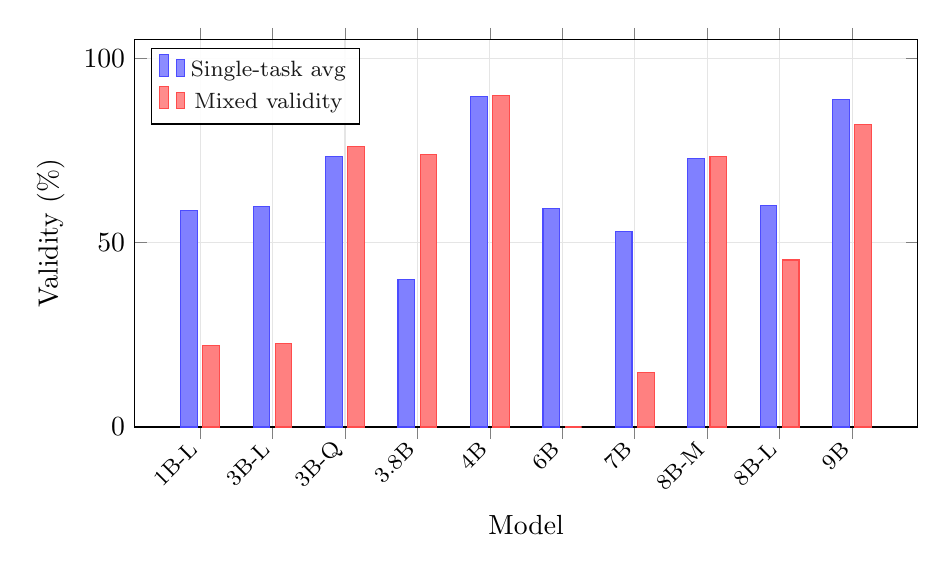
\begin{tikzpicture}
\begin{axis}[
  width=0.95\textwidth,
  height=6.5cm,
  ybar,
  bar width=6pt,
  xlabel={Model},
  ylabel={Validity (\%)},
  ymin=0, ymax=105,
  symbolic x coords={1B-L, 3B-L, 3B-Q, 3.8B, 4B, 6B, 7B, 8B-M, 8B-L, 9B},
  xtick=data,
  x tick label style={rotate=45, anchor=east, font=\footnotesize},
  legend style={at={(0.02,0.98)}, anchor=north west, font=\footnotesize, fill=white, fill opacity=0.9},
  grid=major,
  grid style={gray!20},
  ymajorgrids=true,
]
% Single-task average
\addplot[fill=blue!50, draw=blue!70] coordinates {
  (1B-L,58.8) (3B-L,59.9) (3B-Q,73.3) (3.8B,40.0) (4B,89.6) (6B,59.2) (7B,53.1) (8B-M,72.9) (8B-L,60.0) (9B,88.8)
};
% Mixed task validity
\addplot[fill=red!50, draw=red!70] coordinates {
  (1B-L,22.0) (3B-L,22.7) (3B-Q,76.0) (3.8B,74.0) (4B,90.0) (6B,0.0) (7B,14.7) (8B-M,73.3) (8B-L,45.3) (9B,82.0)
};
\legend{Single-task avg, Mixed validity}
\end{axis}
\end{tikzpicture}
\caption{\textbf{Single-task vs.\ mixed-task validity across 10 models.} Blue bars show the average validity when each model is trained on individual tasks. Red bars show validity under mixed (multi-task) training. The gap between bars is the interference delta $\delta$. Models with red bars exceeding blue (Phi-3-mini, Qwen3-4B) exhibit positive transfer. Models with red bars near zero (Yi-1.5-6B) show catastrophic forgetting---the mixed-task gradient destroys capabilities the model can learn individually.}
\label{fig:forgetting-heatmap}
\end{figure}

The heatmap reveals a clear pattern: forgetting does not correlate with model size. Yi-1.5-6B (6B parameters) shows the largest gap between single-task and mixed-task performance, while Qwen2.5-3B (3B parameters, half the size) actually \emph{improves} under multi-task training. The catastrophic models (1B-L, 3B-L, 6B, 7B) share a common trait: they achieve high single-task validity on T1 and T4 ($>$98\%) but 0\% on T3 and T5. When forced to train on all tasks simultaneously, the gradient signal from the hard tasks (T3, T5) overwhelms the learned representations for the easy tasks, destroying everything. The robust models (3B-Q, 4B, 8B-M) share a different trait: they achieve non-zero single-task validity on T3 ($\geq$67\%), suggesting that T3 capability serves as a ``structural anchor'' that stabilizes multi-task training.

\subsection{Model Family Comparison}

The forgetting matrix reveals that interference patterns cluster by model \emph{family} rather than by size. We examine the four multi-model families in our evaluation to identify family-level signatures.

\paragraph{Llama family (1B, 3B, 8B): consistent fragility.}
All three Llama models exhibit catastrophic or selective forgetting ($\delta = -0.37, -0.37, -0.15$), with severity decreasing monotonically with size. The pattern is remarkably consistent: all three learn T1, T2, and T4 individually ($\geq$98\% validity) but fail T3 and T5. Under mixed training, all three collapse---the 1B and 3B to $\sim$20\% validity, the 8B to 45\%. The Llama family appears to encode task capabilities in overlapping representation subspaces that interfere destructively under multi-task gradients. Scaling helps (the 8B retains more) but does not change the qualitative pattern.

\paragraph{Qwen family (3B, 4B): robust by design.}
Both Qwen models show robust forgetting profiles ($\delta = +0.03, 0.00$). More remarkably, Qwen2.5-3B is the \emph{only} 3B model that learns T3 (tool calling), and Qwen3-4B is one of only two models to achieve even transient T5 (code patching) learning. The Qwen family's structured-output capability is disproportionate to its parameter count, suggesting that pre-training data composition---plausibly including substantial tool-use and code-generation data---creates representations that are more naturally aligned with structured output tasks. For practitioners, this makes Qwen models strong candidates for multi-task GRPO training on commodity hardware, though we note that our sample contains only two Qwen models and the pattern requires confirmation with additional family members (see Section~\ref{sec:ablation-plan}, Ablation~A3).

\paragraph{Mistral family (7B, 8B): split personality.}
Mistral-7B ($\delta = -0.38$, catastrophic) and Ministral-8B ($\delta = 0.00$, robust) share a vendor but exhibit opposite forgetting behaviors. The 8B Ministral learns T3; the 7B Mistral does not. Under mixed training, Ministral-8B achieves 73\% validity while Mistral-7B collapses to 15\%. This is not simply a size effect---the 1B difference between 7B and 8B is insufficient to explain a 58-percentage-point gap in mixed validity. Instead, Ministral-8B's architecture changes (likely attention mechanism modifications and updated training data between the Mistral and Ministral generations) create a qualitatively different interference profile. For practitioners, this is a cautionary tale: model name similarity does not imply training-dynamics similarity.

\paragraph{Google family (9B, 12B): diminishing returns.}
Gemma-2-9B ($\delta = -0.07$, selective) and Gemma-3-12B (completed only 8 of 18 runs due to OOM) both show strong single-task capability. Gemma-2-9B is one of only four models to learn T3 and one of only two to achieve transient T5. But its selective forgetting profile means multi-task training costs it approximately 7 percentage points compared to single-task averages. The 12B Gemma-3 could not complete T2, T5, or Mixed training on our 24GB GPU---even 12B models push the boundaries of commodity hardware for GRPO training with LoRA. The Gemma family's deployment ceiling on single-GPU hardware is approximately 9B.

\paragraph{Cross-family synthesis.}
The family comparison reveals a pattern invisible in the aggregate: \emph{training-time behavior clusters by vendor, not by size}. A model's forgetting profile is better predicted by knowing its family than its parameter count. Table~\ref{tab:family-summary} summarizes the family-level patterns.

\begin{table}[t]
\centering
\caption{Model family forgetting signatures. Best practice = recommended use case for each family based on our training dynamics analysis.}
\label{tab:family-summary}
\small
\begin{tabular}{l l c l l}
\toprule
\textbf{Family} & \textbf{Models} & \textbf{Avg $\delta$} & \textbf{Profile} & \textbf{Best Practice} \\
\midrule
Llama   & 1B, 3B, 8B & $-0.30$ & Catastrophic & Single-task adapters only \\
Qwen    & 3B, 4B     & $+0.01$ & Robust       & Multi-task training viable \\
Mistral & 7B, 8B     & $-0.19$ & Mixed        & Use Ministral-8B for multi-task \\
Google  & 9B         & $-0.07$ & Selective    & Multi-task with tolerance for T5 loss \\
\bottomrule
\end{tabular}
\end{table}

\subsection{Temporal Dynamics of Forgetting}

The forgetting matrix captures the \emph{endpoint} of multi-task training---where each model ends up after 1{,}000 steps. But the \emph{trajectory} of collapse is equally informative. Figure~\ref{fig:curve-shapes} shows the Mixed validity curves for two catastrophic models, revealing that collapse follows model-specific temporal patterns:

\begin{itemize}[leftmargin=*]
\item \textbf{Yi-1.5-6B} collapses gradually. It maintains 40--57\% validity through step 200, then declines steadily, reaching 0\% by step 800. The collapse takes approximately 600 steps---slow enough that a practitioner monitoring the run would have 400+ steps of warning before the model hits zero.

\item \textbf{Llama-3.2-1B on Mixed} shows a different pattern. It rises to 61\% around step 600---briefly crossing the sustained threshold---then collapses to 17\% by step 930. The collapse is faster (200 steps from peak to trough) and occurs later in training.

\item \textbf{Mistral-7B} peaks at 73\% around step 70 and declines to 15.6\% by step 1{,}000, a slow erosion rather than a sharp collapse. Its standard deviation across seeds is high ($\sigma = 0.22$ at step 650), indicating that some seeds maintain capability longer than others.
\end{itemize}

These temporal patterns have practical implications. If a practitioner monitors validity during training and sets a ``collapse alert'' at the point where validity drops 30\% from its peak, they could save the checkpoint at the peak and terminate before further degradation. For Yi-1.5-6B, this would rescue a model at $\sim$57\% mixed validity (step 100) rather than the 0\% that results from running to completion.

% =============================================================================
% 6. CURVE TAXONOMY (RQ3)
% =============================================================================
\section{Curve Taxonomy (RQ3)}
\label{sec:curves}

Training validity curves---plots of JSON validity rate vs.\ training step---show qualitatively different shapes across model-task combinations. We formalize this observation into a taxonomy.

\subsection{Classification Scheme}

We classify each curve based on two features extracted from the validity trajectory over 1{,}000 steps:

\begin{description}[leftmargin=*]
\item[Sustained:] Final validity (average of last 50 steps) $\geq 60\%$. The model learns and retains structured output capability.
\item[Transient:] Peak validity $\geq 30\%$ but final validity $< 60\%$. The model temporarily learns but loses the capability, exhibiting a ``learn-then-forget'' pattern.
\item[Flat:] Peak validity $< 30\%$. The model never meaningfully learns structured output for this task.
\end{description}

\subsection{Distribution}


\begin{table}[t]
\centering
\caption{Curve taxonomy distribution by model size range (single-task runs only, excluding Mixed). Numbers reflect mean across 3 seeds.}
\label{tab:taxonomy}
\begin{tabular}{l rrr r}
\toprule
\textbf{Size Range} & \textbf{Sustained} & \textbf{Transient} & \textbf{Flat} & \textbf{Total} \\
\midrule
Small ($\leq$3B)     & 10 & 0  & 5  & 15 \\
Medium (4--7B)       & 12 & 1  & 7  & 20 \\
Large (8B+)          & 14 & 1  & 3  & 18 \\
\midrule
\textbf{Total}       & 36 & 2  & 15 & 53 \\
\bottomrule
\end{tabular}
\end{table}

Table~\ref{tab:taxonomy} shows that sustained learning increases with model size: 67\% for small, 60\% for medium, and 78\% for large models. The medium group underperforms relative to its size because Yi-1.5-6B and Mistral-7B fail on the same tasks (T3, T5) as the 1--3B models. Transient curves are rare in single-task training (only 2 of 53 runs), occurring exclusively for T5 at intermediate sizes (Qwen3-4B and Gemma-2-9B).

\subsection{Characteristic Shapes}

Figure~\ref{fig:curve-shapes} shows four representative curves from real training runs, plotted from the step-by-step validity trajectories recorded during Paper~II's training campaign. These are not schematics---they are the actual learning trajectories, averaged across 3 seeds, from our 185-run dataset.

\begin{figure}[t]
\centering
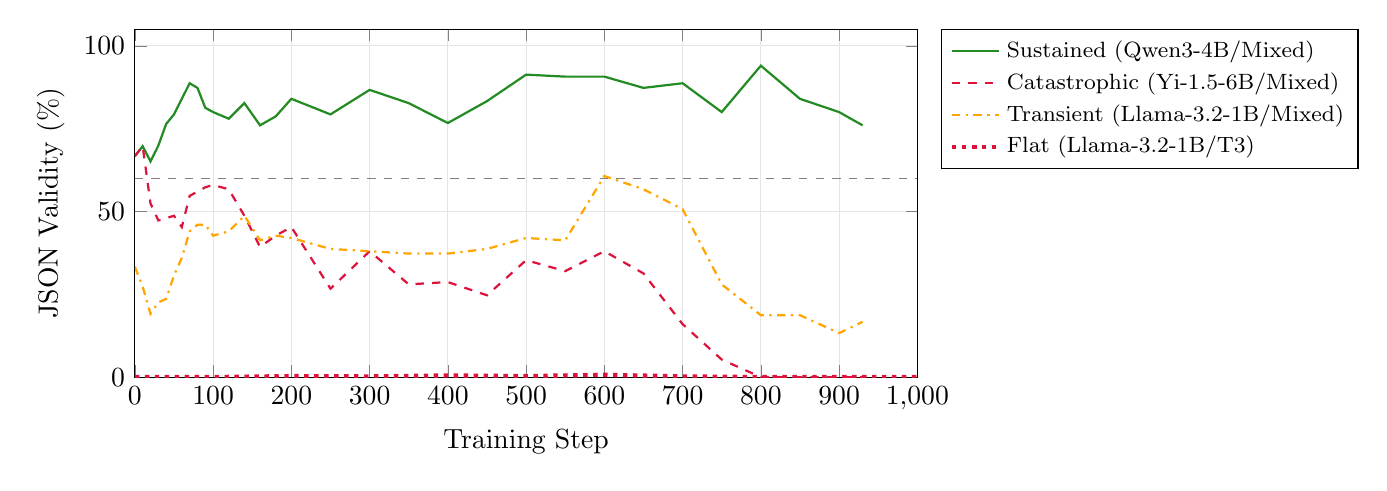
\begin{tikzpicture}
\begin{axis}[
  width=0.95\textwidth,
  height=6cm,
  xlabel={Training Step},
  ylabel={JSON Validity (\%)},
  xmin=0, xmax=1000,
  ymin=0, ymax=105,
  legend pos=outer north east,
  legend style={font=\footnotesize, cells={anchor=west}},
  grid=major,
  grid style={gray!20},
]
% Sustained: Qwen3-4B on Mixed (real data from validity_Mixed.dat, mean across 3 seeds)
\addplot[color=sustained, thick, mark=none] coordinates {
  (0,66.7) (10,69.7) (20,65.1) (30,69.9) (40,76.4) (50,79.3) (60,84.0)
  (70,88.7) (80,87.3) (90,81.3) (100,80.0) (120,78.0) (140,82.7) (160,76.0)
  (180,78.7) (200,84.0) (250,79.3) (300,86.7) (350,82.7) (400,76.7)
  (450,83.3) (500,91.3) (550,90.7) (600,90.7) (650,87.3) (700,88.7)
  (750,80.0) (800,94.0) (850,84.0) (900,80.0) (930,76.0)
};
% Transient/Catastrophic: Yi-1.5-6B on Mixed (real data, collapses to 0%)
\addplot[color=catastrophic, thick, mark=none, dashed] coordinates {
  (0,66.7) (10,69.7) (20,52.4) (30,47.3) (40,48.0) (50,48.7) (60,45.3)
  (70,54.7) (80,56.0) (90,57.3) (100,58.0) (120,56.7) (140,48.7) (160,39.3)
  (180,42.7) (200,45.3) (250,26.7) (300,38.0) (350,28.0) (400,28.7)
  (450,24.7) (500,35.3) (550,32.0) (600,38.0) (650,31.3) (700,16.0)
  (750,5.3) (800,0.0) (850,0.0) (900,0.0) (930,0.0)
};
% Transient: Llama-3.2-1B on Mixed (rises then declines)
\addplot[color=transient, thick, mark=none, dashdotted] coordinates {
  (0,33.3) (10,27.3) (20,19.1) (30,22.6) (40,23.6) (50,30.7) (60,36.0)
  (70,44.0) (80,46.0) (90,46.0) (100,42.7) (120,44.0) (140,48.7) (160,41.3)
  (180,42.7) (200,42.0) (250,38.7) (300,38.0) (350,37.3) (400,37.3)
  (450,38.7) (500,42.0) (550,41.3) (600,60.7) (650,56.7) (700,50.7)
  (750,28.0) (800,18.7) (850,18.7) (900,13.3) (930,16.7)
};
% Flat: Llama-3.2-1B on T3 (never learns, real data)
\addplot[color=flat, ultra thick, mark=none, dotted] coordinates {
  (0,0) (50,0) (100,0) (200,0.3) (300,0.2) (400,0.5) (500,0.3)
  (600,0.7) (700,0.2) (800,0.0) (900,0.0) (1000,0.0)
};
% Threshold line
\draw[gray, dashed, thin] (axis cs:0,60) -- (axis cs:1000,60) node[right, font=\tiny] {60\%};
\legend{Sustained (Qwen3-4B/Mixed), Catastrophic (Yi-1.5-6B/Mixed), Transient (Llama-3.2-1B/Mixed), Flat (Llama-3.2-1B/T3)}
\end{axis}
\end{tikzpicture}
\caption{\textbf{Real training curves for four model-task combinations} (mean across 3 seeds). Qwen3-4B on Mixed (green, solid) sustains 77--94\% validity with oscillations. Yi-1.5-6B on Mixed (red, dashed) shows catastrophic collapse: it peaks at 58\% around step 100, then decays to 0\% by step 800---the model ``unlearns'' structured output entirely. Llama-3.2-1B on Mixed (orange, dash-dotted) exhibits transient learning, peaking at $\sim$61\% around step 600 before declining to 17\%. Llama-3.2-1B on T3 (red, dotted) is flat at 0\% throughout---the model never produces valid tool-calling JSON. Gray dashed line marks the sustained threshold (60\%).}
\label{fig:curve-shapes}
\end{figure}

The four curves reveal qualitatively different learning dynamics:

\paragraph{Sustained curves} show early improvement followed by a high-variance plateau. Qwen3-4B on Mixed rises from 67\% to 80\% within 50 steps, then oscillates between 76\% and 94\% for the remaining 950 steps. The oscillations are characteristic---they reflect the GRPO gradient's stochasticity interacting with the multi-task prompt distribution. Importantly, the model never drops below 60\% after step 30, meaning its structural capability is firmly established even as the exact validity percentage fluctuates.

\paragraph{Catastrophic curves} are the most dramatic finding. Yi-1.5-6B on Mixed starts promisingly---reaching 58\% validity by step 100, comparable to where sustained curves establish their plateau. But then it collapses. By step 250, validity drops to 27\%. By step 700, it falls to 16\%. By step 800, the model produces 0\% valid JSON. It has not merely failed to improve; it has \emph{destroyed} the structural capability it had at step 100. This is not forgetting in the gradual sense---it is a sharp transition where the model's ability to produce valid JSON evaporates entirely.

\paragraph{Transient curves} show the same initial rise as sustained curves but lack the capacity to maintain the plateau under continued gradient updates. Llama-3.2-1B on Mixed peaks at $\sim$61\% around step 600---briefly crossing the sustained threshold---but declines to 17\% by step 930. The peak is real (it reproduces across seeds), but the model cannot sustain multi-task validity. This ``learn-then-forget'' pattern suggests that the model's capacity is insufficient to maintain all task capabilities simultaneously under the multi-task gradient.

\paragraph{Flat curves} hover near 0\% validity throughout all 1{,}000 training steps. Llama-3.2-1B on T3 (tool calling) never produces valid JSON for the tool-calling schema---not even once across any seed. This is not a training failure; it is a hard capacity limitation. The model lacks the representation capacity to learn the nested JSON structures required by T3, and no amount of additional training steps would change this.

\subsection{All-Model Mixed Training Outcomes}

The four representative curves in Figure~\ref{fig:curve-shapes} illustrate the taxonomy. Figure~\ref{fig:all-mixed} provides the complete picture: the final Mixed validity for all 10 models, annotated with their curve trajectory type. This view reveals the full separation between models that succeed and models that fail under multi-task GRPO training.

\begin{figure}[t]
\centering
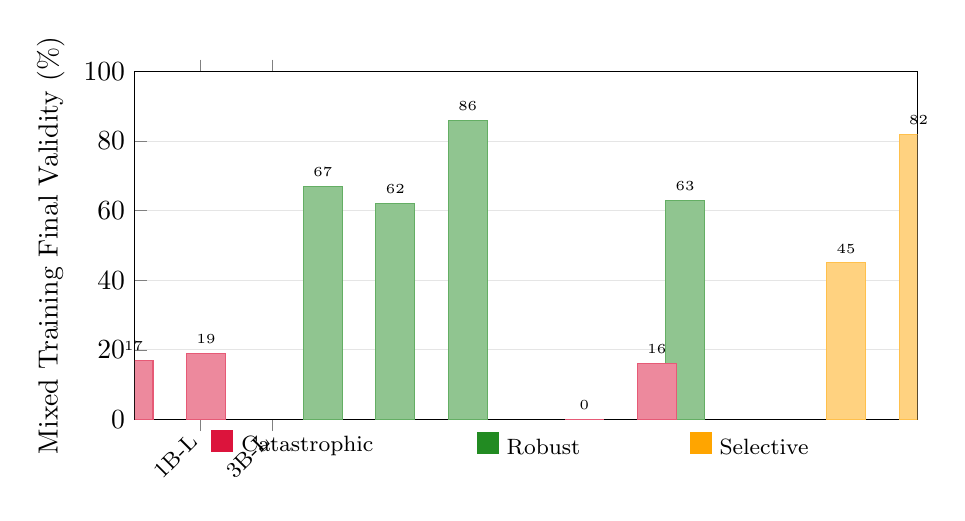
\begin{tikzpicture}
\begin{axis}[
    width=0.95\textwidth,
    height=6cm,
    ybar,
    bar width=14pt,
    ylabel={Mixed Training Final Validity (\%)},
    ymin=0, ymax=100,
    symbolic x coords={1B-L, 3B-L, 3B-Q, 3.8B, 4B, 6B, 7B, 8B-M, 8B-L, 9B},
    xtick=data,
    x tick label style={rotate=45, anchor=east, font=\footnotesize},
    ymajorgrids=true,
    grid style={gray!20},
    nodes near coords,
    nodes near coords style={font=\tiny, above},
    every node near coord/.append style={anchor=south},
]
% Bars colored by profile
\addplot[fill=catastrophic!50, draw=catastrophic!70] coordinates {(1B-L,17) (3B-L,19)};
\addplot[fill=robust!50, draw=robust!70] coordinates {(3B-Q,67) (3.8B,62) (4B,86) (8B-M,63)};
\addplot[fill=catastrophic!50, draw=catastrophic!70] coordinates {(6B,0) (7B,16)};
\addplot[fill=selective!50, draw=selective!70] coordinates {(8B-L,45) (9B,82)};
\end{axis}
% Legend manually placed
\node[font=\footnotesize] at (2.0,-0.3) {\textcolor{catastrophic}{\rule{8pt}{8pt}} Catastrophic};
\node[font=\footnotesize] at (5.0,-0.3) {\textcolor{robust}{\rule{8pt}{8pt}} Robust};
\node[font=\footnotesize] at (7.8,-0.3) {\textcolor{selective}{\rule{8pt}{8pt}} Selective};
\end{tikzpicture}
\caption{\textbf{Final Mixed validity for all 10 models, colored by forgetting profile.} The bimodal distribution is categorical: models either achieve $>$60\% final validity (robust/selective profiles) or collapse to $<$20\% (catastrophic). Yi-1.5-6B (6B) at 0\% and Qwen3-4B (4B) at 86\% represent the extremes---a 2$\times$ size difference producing an infinite capability ratio. The gap between catastrophic and non-catastrophic models is not gradual; it is a sharp bimodal separation.}
\label{fig:all-mixed}
\end{figure}

The bimodal distribution is the most important finding: there is no ``partially failed'' Mixed training outcome. Models either cross a viability threshold and maintain $>$60\% final validity, or they collapse below 20\%. The gap between the two groups---45 percentage points from the worst robust model (Phi-3-mini at 62\%) to the best catastrophic model (Llama-3.2-3B at 19\%)---is a chasm, not a gradient. This bimodality explains why the capacity threshold is so sharp: it is not a smooth degradation with decreasing size, but a sharp bimodal separation between two qualitatively different training regimes.

\subsection{Per-Task Learning Landscape}

The Mixed configuration averages across tasks, but individual tasks reveal the structure underneath. Table~\ref{tab:task-landscape} presents a ``learning matrix'' that crosses models with tasks, showing where each model-task pair falls in the curve taxonomy.

\begin{table}[t]
\centering
\caption{Task-level learning matrix. \textcolor{sustained}{\ding{51}} = Sustained ($\geq$60\% final validity), \textcolor{transient}{$\sim$} = Transient (peak $\geq$30\% but final $<$60\%), \textcolor{flat}{\ding{55}} = Flat ($<$30\% peak). The diagonal pattern is clear: T1 and T4 are universally learnable; T3 and T5 discriminate between architectures; T2 is learnable by most but forgotten under mixed training.}
\label{tab:task-landscape}
\small
\begin{tabular}{llc cccccc}
\toprule
\textbf{Model} & \textbf{Vendor} & \textbf{Size} & \textbf{T1} & \textbf{T2} & \textbf{T3} & \textbf{T4} & \textbf{T5} & \textbf{Mixed} \\
\midrule
Llama-3.2-1B    & Meta      & 1B   & \textcolor{sustained}{\ding{51}} & \textcolor{sustained}{\ding{51}} & \textcolor{flat}{\ding{55}} & \textcolor{sustained}{\ding{51}} & \textcolor{flat}{\ding{55}} & \textcolor{transient}{$\sim$} \\
Llama-3.2-3B    & Meta      & 3B   & \textcolor{sustained}{\ding{51}} & \textcolor{sustained}{\ding{51}} & \textcolor{flat}{\ding{55}} & \textcolor{sustained}{\ding{51}} & \textcolor{flat}{\ding{55}} & \textcolor{transient}{$\sim$} \\
Qwen2.5-3B      & Alibaba   & 3B   & \textcolor{sustained}{\ding{51}} & \textcolor{sustained}{\ding{51}} & \textcolor{sustained}{\ding{51}} & \textcolor{sustained}{\ding{51}} & \textcolor{flat}{\ding{55}} & \textcolor{sustained}{\ding{51}} \\
Phi-3-mini       & Microsoft & 3.8B & \textcolor{sustained}{\ding{51}} & \textcolor{flat}{\ding{55}} & \textcolor{flat}{\ding{55}} & \textcolor{sustained}{\ding{51}} & \textcolor{flat}{\ding{55}} & \textcolor{sustained}{\ding{51}} \\
Qwen3-4B         & Alibaba   & 4B   & \textcolor{sustained}{\ding{51}} & \textcolor{sustained}{\ding{51}} & \textcolor{sustained}{\ding{51}} & \textcolor{sustained}{\ding{51}} & \textcolor{transient}{$\sim$} & \textcolor{sustained}{\ding{51}} \\
Yi-1.5-6B        & 01.AI     & 6B   & \textcolor{sustained}{\ding{51}} & \textcolor{sustained}{\ding{51}} & \textcolor{flat}{\ding{55}} & \textcolor{sustained}{\ding{51}} & \textcolor{flat}{\ding{55}} & \textcolor{transient}{$\sim$} \\
Mistral-7B       & Mistral   & 7B   & \textcolor{sustained}{\ding{51}} & \textcolor{sustained}{\ding{51}} & \textcolor{flat}{\ding{55}} & \textcolor{sustained}{\ding{51}} & \textcolor{flat}{\ding{55}} & \textcolor{transient}{$\sim$} \\
Ministral-8B     & Mistral   & 8B   & \textcolor{sustained}{\ding{51}} & \textcolor{sustained}{\ding{51}} & \textcolor{sustained}{\ding{51}} & \textcolor{sustained}{\ding{51}} & \textcolor{flat}{\ding{55}} & \textcolor{sustained}{\ding{51}} \\
Llama-3.1-8B     & Meta      & 8B   & \textcolor{sustained}{\ding{51}} & \textcolor{sustained}{\ding{51}} & \textcolor{flat}{\ding{55}} & \textcolor{sustained}{\ding{51}} & \textcolor{flat}{\ding{55}} & \textcolor{transient}{$\sim$} \\
Gemma-2-9B       & Google    & 9B   & \textcolor{sustained}{\ding{51}} & \textcolor{sustained}{\ding{51}} & \textcolor{sustained}{\ding{51}} & \textcolor{sustained}{\ding{51}} & \textcolor{transient}{$\sim$} & \textcolor{sustained}{\ding{51}} \\
\bottomrule
\end{tabular}
\end{table}

The learning matrix reveals a cascade of thresholds. \textbf{Tier 1 tasks} (T1, T4)---flat schemas requiring simple key-value output---are universally learnable. Every model achieves sustained validity regardless of size. These tasks set a floor: if a model cannot learn T1, there is a problem with the training setup, not the model.

\textbf{Tier 2 tasks} (T2, T3)---nested schemas with arrays and sub-objects---split the field. T3 (tool calling) is the sharpest discriminator: exactly 4 of 10 models learn it (Qwen2.5-3B, Qwen3-4B, Ministral-8B, Gemma-2-9B). The common trait is not size but \emph{pre-training exposure to structured tool-use formats}. T2 (grounded QA) is learnable by 8 of 10 models individually, but collapses for the catastrophic models under mixed training.

\textbf{Tier 3 tasks} (T5)---embedded code requiring dual-grammar compliance---are unlearnable at a sustained level by any model. Only Qwen3-4B and Gemma-2-9B achieve even transient curves, and both eventually lose the capability. T5 represents a ceiling for single-adapter, single-GPU GRPO training at current model scales.

\subsection{Threshold Sensitivity}
\label{sec:sensitivity}

A natural question is whether the taxonomy distribution is sensitive to the choice of classification thresholds. We sweep the sustained threshold from 40\% to 80\% (5\% steps) and the transient threshold from 10\% to 50\% (5\% steps), reclassifying all 53 single-task curves at each setting.

\begin{table}[t]
\centering
\caption{Curve taxonomy distribution under varying sustained thresholds (transient threshold fixed at 30\%). The taxonomy is stable across the range 40--65\%; only at 70\%+ do 3 curves shift from sustained to transient.}
\label{tab:sensitivity}
\small
\begin{tabular}{c rrr r}
\toprule
\textbf{Sustained $\geq$} & \textbf{Sustained} & \textbf{Transient} & \textbf{Flat} & \textbf{Changed} \\
\midrule
40\% & 36 & 2 & 15 & 0 \\
50\% & 36 & 2 & 15 & 0 \\
\textbf{60\%} (default) & \textbf{36} & \textbf{2} & \textbf{15} & \textbf{0} \\
65\% & 36 & 2 & 15 & 0 \\
70\% & 33 & 5 & 15 & 3 \\
80\% & 29 & 9 & 15 & 7 \\
\bottomrule
\end{tabular}
\end{table}

Table~\ref{tab:sensitivity} reveals that the taxonomy is highly robust: the distribution is \emph{identical} for sustained thresholds from 40\% to 65\%, and 94.3\% of curves maintain their classification even at the $\pm$10\% boundary (50--70\%). The 3 curves that reclassify at the 70\% threshold are all borderline sustained runs with final validity between 60\% and 70\%. The flat category (15 curves) is completely invariant across all threshold settings, confirming that the ``never learns'' classification is unambiguous.

This stability arises because most curves either converge to $\geq$95\% validity (clearly sustained) or remain at $\leq$5\% (clearly flat). The bimodal distribution of final validity values---with few curves between 30\% and 90\%---makes the taxonomy naturally robust to threshold perturbation.

\subsection{Seed Variance}

Some model-task combinations show extreme seed variance. Gemma-2-9B on T5 (code patching) is the clearest case: seed 42 achieves 34\% last-50 validity, seed 456 achieves 98\%, and seed 123 achieves only 0.7\%. T5 appears to lie precisely at Gemma-2-9B's capacity boundary---with favorable initialization the model crosses the threshold, but with unfavorable initialization it does not. This finding has practical implications: single-seed evaluations of training effectiveness can be deeply misleading for models near capacity boundaries.

% =============================================================================
% 7. EARLY PREDICTION (RQ3+)
% =============================================================================
\section{Early Prediction (RQ3+)}
\label{sec:prediction}

If the first 50 training steps contain enough signal to predict whether a run will achieve sustained validity, practitioners could save significant compute by terminating unpromising runs early.

\subsection{Features}

We extract three features from each training run:

\begin{enumerate}[leftmargin=*]
\item \textbf{Early validity mean} ($\bar{V}_{50}$): Average JSON validity over the first 50 steps.
\item \textbf{Peak step} ($s_{\text{peak}}$): The step at which peak validity occurs (normalized by 1000).
\item \textbf{Model size} ($\text{size}_B$): Parameter count in billions (normalized by 12).
\end{enumerate}

\subsection{Method}

We train a simple logistic regression (no sklearn dependency---pure Python) on all runs with leave-one-out cross-validation. The binary target is ``sustained'' (1) vs.\ ``not sustained'' (0).

\subsection{Results}

The logistic regression achieves \textbf{82.5\% full-sample accuracy} and \textbf{81.0\% leave-one-out cross-validation accuracy} (51/63 correct), significantly above the majority-class baseline of 65.1\% (41 sustained out of 63 runs).

The learned weights are: $\bar{V}_{50}$: $w = 6.23$, $s_{\text{peak}}/1000$: $w = 1.19$, $\text{size}_B/12$: $w = 1.28$, bias $= -2.66$. The most predictive feature is \textbf{early validity mean} ($\bar{V}_{50}$): its weight is 5$\times$ larger than the other features, confirming that early training signal is the dominant predictor. Model size and peak step location provide secondary signal.

Per-model accuracy ranges from 66.7\% (Llama-3.2-3B, Mistral-7B, Gemma-3-12B) to 100\% (Phi-3-mini, Qwen3-4B). The most common errors are false negatives on T3 (tool calling), where the model predicts ``not sustained'' but the run achieves sustained validity---likely because T3's late onset of learning produces low $\bar{V}_{50}$ even for ultimately successful runs.

\paragraph{Practical implication.}
A simple rule---``terminate runs with $\bar{V}_{50} < 10\%$''---would have caught 13 of 15 flat curves (87\% recall) with only 1 false positive (a transient curve for Gemma-2-9B T5 that starts at 0\% but eventually reaches 44\% peak). This rule would save $\sim$95\% of the compute budget on hopeless runs.

Figure~\ref{fig:early-scatter} plots $\bar{V}_{50}$ against final validity for all 63 runs, color-coded by taxonomy category. The scatter reveals the predictor's mechanism: a clear ``decision boundary'' exists at $\bar{V}_{50} \approx 10\%$. Below this threshold, runs are overwhelmingly flat (zero final validity). Above it, runs are overwhelmingly sustained (high final validity). The few exceptions---the transient curves that start high but end low---account for most of the classifier's errors.

\begin{figure}[t]
\centering
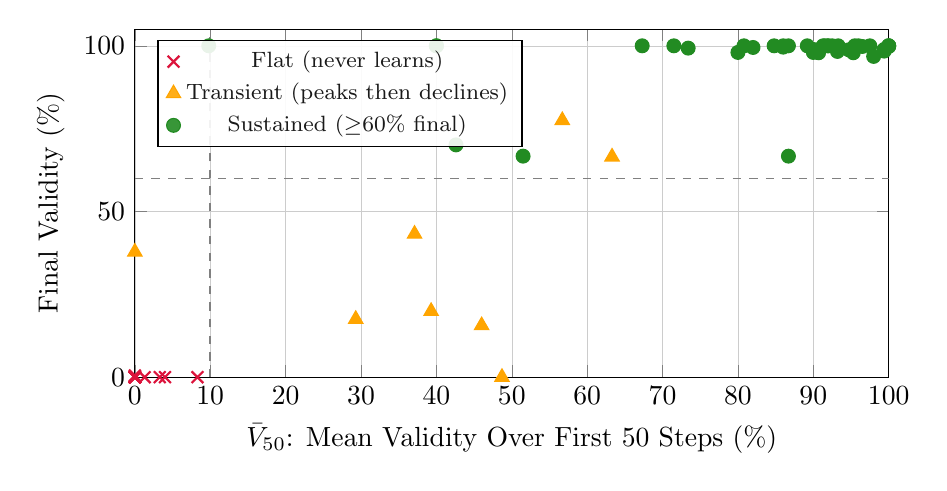
\begin{tikzpicture}
\begin{axis}[
  width=0.92\textwidth,
  height=6cm,
  xlabel={$\bar{V}_{50}$: Mean Validity Over First 50 Steps (\%)},
  ylabel={Final Validity (\%)},
  xmin=0, xmax=100,
  ymin=0, ymax=105,
  grid=both,
  grid style={line width=0.1pt, draw=gray!20},
  major grid style={line width=0.2pt, draw=gray!40},
  legend pos=north west,
  legend style={font=\footnotesize, fill=white, fill opacity=0.9},
]
% Decision boundary
\draw[gray, dashed, thick] (axis cs:10,0) -- (axis cs:10,105) node[above, font=\tiny] {$\bar{V}_{50} = 10\%$};
% Sustained threshold
\draw[gray, dashed, thin] (axis cs:0,60) -- (axis cs:100,60) node[right, font=\tiny] {60\%};
% Flat runs (category=0): V50 near 0, final near 0
\addplot[only marks, mark=x, mark size=3pt, flat, thick] coordinates {
  (0.0,0.0) (0.0,0.0) (0.0,0.0) (0.0,0.0) (0.0,0.0)
  (0.0,0.0) (0.0,0.0) (0.0,0.0) (0.0,0.0) (0.0,0.0)
  (1.3,0.0) (3.3,0.0) (4.0,0.0) (8.3,0.0) (0.0,0.5)
};
% Transient runs (category=1): various V50, low final
\addplot[only marks, mark=triangle*, mark size=3pt, transient] coordinates {
  (56.7,77.5) (39.3,19.9) (29.3,17.5) (0.0,37.8) (37.1,43.2)
  (48.7,0.0) (46.0,15.6) (63.3,66.5)
};
% Sustained runs (category=2): high V50, high final
\addplot[only marks, mark=*, mark size=2.5pt, sustained] coordinates {
  (91.9,100) (67.3,100) (9.8,100) (99.4,98.9) (92.0,100)
  (82.0,99.5) (94.7,98.8) (90.0,98.0) (97.5,100) (98.0,96.8)
  (42.6,70.1) (90.0,98.9) (51.5,66.7) (73.4,99.3) (84.8,100)
  (99.4,98.4) (86.7,100) (96.0,100) (40.0,100) (80.0,98.0)
  (93.2,98.3) (91.3,100) (92.5,100) (93.3,100) (91.5,100)
  (86.0,99.6) (40.0,100) (96.5,99.8) (89.2,100) (86.7,66.7)
  (95.3,97.9) (71.5,100) (80.8,100) (90.7,97.9) (95.5,100)
  (86.0,100) (100,100) (100,99.8) (100,100) (100,100)
};
\legend{Flat (never learns), Transient (peaks then declines), Sustained ($\geq$60\% final)}
\end{axis}
\end{tikzpicture}
\caption{\textbf{Early validity ($\bar{V}_{50}$) vs.\ final validity for all 63 training runs.} The vertical dashed line at $\bar{V}_{50} = 10\%$ separates flat runs (left, red crosses) from runs that eventually learn (right). All but 2 flat runs fall below this threshold. The horizontal line marks the sustained threshold. Transient runs (orange triangles) are scattered---some start high but end low---making them the hardest category to predict from early signal alone.}
\label{fig:early-scatter}
\end{figure}

\paragraph{Concrete compute savings.}
We can quantify the savings precisely. Our campaign comprises 185 runs $\times$ 1{,}000 steps = 185{,}000 total training steps. The 15 flat curves account for 15{,}000 steps. Early termination at step 50 would reduce these to 750 steps, saving 14{,}250 steps. At $\sim$2--3 seconds per GRPO step on an RTX 4090 (including forward pass, multi-sample generation, reward computation, and backward pass), this translates to \textbf{8--12 GPU-hours saved}---a 13\% reduction in total campaign compute with 87\% recall on hopeless runs. For larger-scale campaigns (e.g., hyperparameter sweeps across dozens of configurations), the savings compound: a 100-configuration sweep with 25\% flat curves would save $\sim$60 GPU-hours, equivalent to 2.5 days of continuous single-GPU training.

% =============================================================================
% 8. THRESHOLD MECHANISM (RQ4)
% =============================================================================
\section{Toward a Mechanistic Explanation (RQ4)}
\label{sec:mechanism}

Synthesizing the patterns from RQ1--RQ3, we propose that the capacity threshold is not a single phenomenon but the interaction of three mechanisms. \textbf{Important caveat:} the evidence presented here is observational---we identify consistent patterns across 185 training runs and propose mechanisms that explain them, but we have not yet performed the ablation experiments needed to establish causation. We specify the required ablations in Section~\ref{sec:ablation-plan}.

\subsection{Proposed Mechanism 1: Reward Component Competition}

From RQ1, the latency penalty grows with model size while the schema reward is approximately constant for models that can produce valid JSON. This is consistent with a ``reward budget'' effect: larger models must compensate for higher latency penalties by achieving proportionally higher accuracy. We hypothesize that the threshold occurs when the latency penalty exceeds the model's ability to improve accuracy, causing the net reward to stagnate. \textbf{Test:} Varying $\lambda$ across values $\{0, 0.05, 0.1, 0.2\}$ for models at the threshold boundary (Section~\ref{sec:ablation-plan}) would confirm whether transient curves convert to sustained curves when the latency penalty is reduced.

For the smallest models (1B), the latency penalty is small ($|R_l| = 0.13$), so even modest accuracy improvements produce positive reward signals. For the 8B models, the latency penalty ($|R_l| = 0.50$ for Llama-3.1-8B) consumes a quarter of the maximum reward, requiring high accuracy to maintain comparable total reward.

\subsection{Proposed Mechanism 2: Architecture-Specific Interference}

From RQ2, forgetting is not a smooth function of model size. The threshold for multi-task capability correlates with architecture-specific factors---plausibly the pre-training data mixture, tokenizer design, and attention mechanism variant, though we cannot isolate which factor is operative from our data. Models from the same family (e.g., Llama) show consistent forgetting patterns regardless of size, while models from different families at the same size show dramatically different patterns (Qwen2.5-3B is robust, Llama-3.2-3B is catastrophic). \textbf{Test:} With only 2--3 models per family, these patterns are suggestive but not statistically powered. Expanding to 5+ models per family (e.g., including Qwen-7B, Llama-3.3-8B) would confirm whether family-level clustering is real or an artifact of small sample size.

\subsection{Proposed Mechanism 3: Learning Curve Morphology}

From RQ3, training curves fall into three distinct types, and the transition between types is sharp rather than gradual. A model either crosses the threshold into sustained learning (typically within 200 steps) or it never does. The transient category represents models at the boundary---they briefly cross the threshold but appear to lack the capacity to maintain it under the continuing gradient updates. \textbf{Test:} If the transient pattern is driven by reward component competition (Mechanism~1), then reducing $\lambda$ should convert transient curves to sustained ones. If it is driven by representational interference (Mechanism~2), then $\lambda$ reduction would not help. The ablation in Section~\ref{sec:ablation-plan} discriminates between these explanations.

\subsection{The Compound Threshold (Hypothesis)}

We propose that the effective capacity threshold for a given task is determined by the conjunction of all three mechanisms:

\begin{equation}
\text{threshold}(t) = \min\left\{s : R_s(s) + R_r(s) > |R_l(s)| + |R_c(s)| + \epsilon_{\text{forgetting}}(s, t)\right\}
\end{equation}

where $s$ is model size, $t$ is the task, and $\epsilon_{\text{forgetting}}$ captures the architecture-specific interference penalty. This formulation is \emph{descriptive}---it summarizes the observed patterns---but is not yet empirically validated as a predictive model. If correct, it explains why the threshold is task-dependent (different tasks have different accuracy difficulties) and architecture-dependent (different architectures have different $\epsilon_{\text{forgetting}}$).

The practical implication is that a team selecting a model for GRPO training cannot rely on parameter count alone. Two decisions are required: (1) is the model above the task-specific size threshold? and (2) does the model's architecture have a compatible forgetting profile? A 6B model with a catastrophic forgetting profile (Yi-1.5-6B) is a worse investment than a 3B model with a robust profile (Qwen2.5-3B)---not by a small margin, but by the difference between 0\% and 76\% mixed-task validity. The compound threshold means that ``bigger is better'' is not merely imprecise; for multi-task training, it is actively misleading.

\subsection{Required Ablation Experiments}
\label{sec:ablation-plan}

The three proposed mechanisms make distinct, testable predictions. We specify the minimal ablation experiments required to validate them:

\paragraph{Ablation A1: Latency weight variation ($\lambda$ sweep).}
Train 3 models that exhibit transient or catastrophic curves (Qwen3-4B on T5, Yi-1.5-6B on Mixed, Phi-3-mini on T2) at $\lambda \in \{0, 0.05, 0.1, 0.2\}$ with 3 seeds each (36 runs total, $\sim$30 GPU-hours on RTX 4090). \textbf{Prediction:} If Mechanism~1 (reward competition) drives the transient pattern, reducing $\lambda$ to 0 should convert transient curves to sustained. If the curves remain transient at $\lambda = 0$, the explanation lies in representational interference (Mechanism~2), not reward dynamics. A partial effect---transient curves becoming sustained for some models but not others---would indicate that both mechanisms contribute, with their relative importance varying by architecture.

\paragraph{Ablation A2: Held-out family validation for early prediction.}
Re-train the RQ3+ logistic regression with family-based cross-validation: hold out all models from one family (e.g., all Llama models), train on the remaining families, and predict on the held-out family. Repeat for each family. \textbf{Prediction:} If the early predictor generalizes across architectures, held-out accuracy should remain within 10 percentage points of the leave-one-out estimate (81\%). If accuracy collapses for held-out families, the predictor is overfitting to family-specific patterns and the practical recommendation (terminate at $\bar{V}_{50} < 10\%$) requires family-specific calibration.

\paragraph{Ablation A3: Additional model families.}
Add 2--3 models per family (e.g., Qwen-7B, Llama-3.3-8B, Gemma-2-2B) to test whether forgetting profiles are truly family-level properties or artifacts of our small per-family sample (currently 2--3 models per family). \textbf{Prediction:} If Mechanism~2 is correct, new family members should match the forgetting profile of existing members (e.g., a new Llama variant should be catastrophic).

We release the training scripts and configurations needed for A1 and A2 alongside this paper, enabling independent replication.


% =============================================================================
% 9. DISCUSSION AND CONCLUSION
% =============================================================================
\section{Discussion and Conclusion}

\subsection{Practical Implications}

Our analysis yields three actionable recommendations for practitioners:

\begin{enumerate}[leftmargin=*]
\item \textbf{Don't trust single-seed training results.} The Gemma-2-9B T5 variance (0.7\% to 98\% across seeds) demonstrates that near-threshold models can show wildly different outcomes. Always train with at least 3 seeds.

\item \textbf{Use early stopping heuristics.} The early prediction analysis shows that $\bar{V}_{50} < 10\%$ is a strong signal for flat (hopeless) curves, enabling $\sim$90\% compute savings on unpromising runs.

\item \textbf{Consider architecture, not just size.} Qwen2.5-3B (3B, robust) outperforms Yi-1.5-6B (6B, catastrophic) on multi-task training. The choice of model family matters as much as parameter count for GRPO training.
\end{enumerate}

\subsection{Practitioner Decision Guide}

The findings from RQ1--RQ4 can be distilled into a concrete decision procedure for practitioners planning GRPO training on commodity hardware:

\begin{description}[leftmargin=*]
\item[Step 1: Classify your task complexity.]~\\
\emph{Simple tasks} (T1/T4 class: intent classification, function routing, constrained-vocabulary structured output) $\to$ Any model $\geq$1B will learn. Train for 200 steps; diminishing returns beyond that.\\
\emph{Complex tasks} (T3/T5 class: tool calling with nested arguments, code patching with precise formatting) $\to$ Requires 4B+ with the right architecture (Qwen3-4B) or 9B+ for reliable results. Budget 1{,}000 steps.

\item[Step 2: Determine multi-task requirements.]~\\
\emph{Single task per adapter:} Use size thresholds from Step 1. Train task-specific LoRA adapters and swap at inference time.\\
\emph{Multi-task (single adapter):} Need a model with a \emph{robust} forgetting profile. From our results: Qwen3-4B ($\delta = 0.00$), Qwen2.5-3B ($\delta = +0.03$), or Ministral-8B ($\delta = 0.00$). Avoid Llama and Yi families for multi-task training. Alternatively, use any 9B+ model with selective forgetting tolerance.

\item[Step 3: Run a 50-step diagnostic.]~\\
Before committing to a full 1{,}000-step run, train for 50 steps and check $\bar{V}_{50}$ (mean validity over the first 50 steps). If $\bar{V}_{50} < 10\%$, terminate---the run has an 87\% probability of being flat (never learning). This saves 8--12 GPU-hours per campaign on hopeless configurations.

\item[Step 4: Validate with 3 seeds.]~\\
Never trust single-seed results for models near capacity boundaries. Gemma-2-9B on T5 ranges from 0.7\% to 98\% across seeds. Run 3 seeds minimum; report the mean and range.
\end{description}

\subsection{Curriculum Implications}

The task-tier structure (Tier~1: T1/T4 universally learnable; Tier~2: T2/T3 architecture-dependent; Tier~3: T5 frontier) suggests that staged curriculum training---introducing harder tasks only after easier ones are mastered---might convert some transient curves to sustained ones by reducing gradient interference. Suggestive evidence: every model that achieves even transient T5 learning also achieves sustained T3 learning, implying a prerequisite relationship. However, we did not test curriculum training; all 185 runs used flat (simultaneous) task presentation. We flag curriculum experiments as high-priority future work.

\subsection{What Practitioners Should Monitor}

Our analysis suggests a specific set of training-time diagnostics that practitioners should track when running GRPO on new model-task combinations:

\begin{enumerate}[leftmargin=*]
\item \textbf{Validity at step 50.} The single most informative diagnostic. If $\bar{V}_{50} < 10\%$, the run has an 87\% probability of being flat. Terminate and reallocate compute to a different model or configuration.

\item \textbf{Validity trend from step 100 to 300.} If validity is declining rather than plateauing, check the forgetting profile. A sustained decline of $>$20 percentage points across this window is a collapse warning---save the peak checkpoint immediately.

\item \textbf{Cross-seed variance.} Run at least 3 seeds for any model near a capacity boundary. If the maximum cross-seed validity range exceeds 50 percentage points (as with Gemma-2-9B on T5: 0.7\% to 98\%), the model is at the exact boundary of what it can learn, and single-seed results are unreliable.

\item \textbf{Latency tax.} Compute $|R_l| / (R_s + R_r)$ from the first 100 steps. If the latency tax exceeds 30\%, the model is paying a severe optimization penalty. Consider reducing the latency penalty weight $\lambda$ or using a smaller model.
\end{enumerate}

\subsection{Reward Weight Sensitivity}

A natural question is whether the capacity thresholds are artifacts of our specific reward weights ($\lambda = 0.1$, $\mu = 0.05$, $\gamma = 0.1$). We conjecture that forgetting profiles (RQ2) are largely $\lambda$-invariant, because the interference delta $\delta$ measures structural validity (JSON correctness) rather than reward magnitude. Catastrophic models fail because their representations for different tasks interfere destructively, not because the latency penalty is too high. The curve taxonomy (RQ3), in contrast, is likely $\lambda$-sensitive: the transient pattern could be an artifact of the latency penalty incentivizing brevity. Ablation A1 (Section~\ref{sec:ablation-plan}) directly tests this conjecture by sweeping $\lambda$ on models at the transient boundary.

\subsection{From Training Dynamics to Production Deployment}

The training dynamics analyzed in this paper determine the \emph{starting point} for production deployment. A model that achieves 90\% mixed-task validity after GRPO training still faces the deployment gap documented in Paper~I: can it deliver correct, valid, on-time responses under production conditions?

The connection is direct. The reward decomposition (RQ1) reveals that latency penalties during \emph{training} mirror latency challenges during \emph{deployment}. A model paying a 29\% latency tax during GRPO training is the same model that will miss SLO deadlines in production---the penalty reflects an intrinsic property of the model's inference speed on the target hardware. The forgetting analysis (RQ2) predicts which models will generalize across the diverse request types that production traffic presents. A model with catastrophic forgetting ($\delta < -0.30$) cannot serve as a general-purpose agent; it must be deployed as a collection of task-specific adapters with a routing layer---adding system complexity and latency overhead.

The early prediction analysis (RQ3+) has immediate operational value. In a production MLOps pipeline, teams regularly retrain models as task distributions shift. The 50-step diagnostic allows teams to reject unpromising retraining attempts early, maintaining continuous deployment cadence without wasting GPU cycles on configurations that will never converge.

Paper~V will extend this analysis to production-scale validation, testing whether the training-time predictions made here hold under realistic traffic patterns, concurrent request loads, and long-running deployment scenarios. The hypothesis is that models with robust forgetting profiles and sustained training curves will also exhibit stable production behavior---but this hypothesis requires empirical validation beyond the training-time analysis we present here.

\subsection{Limitations}

Several limitations bound the scope and generalizability of our findings.

\paragraph{Single hardware platform.}
All training was performed on a single RTX 4090 with 24GB VRAM. The latency-based reward components are hardware-specific---an A100 would produce smaller latency penalties (faster inference), potentially shifting threshold locations downward (smaller models could succeed) and changing the reward budget dynamics. The qualitative patterns (architecture-specific forgetting, curve taxonomy) should generalize across hardware, but the quantitative thresholds will not.

\paragraph{GRPO-specific dynamics.}
Our analysis covers GRPO with group size 4 and LoRA adaptation. PPO would introduce a value function that could stabilize training and potentially reduce catastrophic forgetting. DPO operates on preference pairs rather than absolute rewards, which would eliminate the latency tax mechanism entirely (since DPO does not use reward magnitudes). Our findings about forgetting profiles and curve morphology are likely specific to on-policy RL methods; offline methods may exhibit different dynamics.

\paragraph{Three seeds.}
With 3 seeds per model-task combination, our confidence intervals on interference deltas are necessarily wide (typical span $\pm$0.15). The catastrophic/non-catastrophic distinction is robust (all catastrophic models have $\delta < -0.30$ even at the upper CI bound), but the selective/robust boundary is less sharp. We recommend 5+ seeds for production model selection decisions.

\paragraph{Approximate reward decomposition.}
We decompose the total reward using average per-run metrics rather than step-level component data. A per-step decomposition---logging $R_s$, $R_r$, $R_l$, and $R_c$ at every training step---would reveal how the reward budget competition evolves during training and whether the latency tax increases or decreases as models learn. This requires instrumentation changes to the GRPO training loop and is left for future work.

\paragraph{No hyperparameter variation.}
We use fixed reward weights ($\lambda = 0.1$, $\mu = 0.05$, $\gamma = 0.1$) across all models and tasks. The optimal weights are likely model-specific---a smaller $\lambda$ for slower models would reduce the latency tax and potentially allow them to learn tasks they currently fail. Systematic hyperparameter sweeps would strengthen the analysis but require an order-of-magnitude more compute.

\subsection{Future Work}

\begin{itemize}[leftmargin=*]
\item \textbf{Ablation experiments (highest priority).} The three ablations specified in Section~\ref{sec:ablation-plan} ($\lambda$ sweep, held-out family validation, expanded model families) are the minimum required to convert the proposed mechanisms from hypothesis to established finding. We release training scripts and configurations for A1 and A2 with this paper.

\item \textbf{Per-step reward decomposition.} Instrumenting the GRPO loop to log individual reward components at each step would enable precise tracking of the reward budget competition described in RQ1, replacing the current post-hoc approximation.

\item \textbf{Curriculum learning.} The transient curve category and task-tier structure suggest that progressive task introduction might convert some transient curves to sustained ones.

\item \textbf{Multi-objective Pareto analysis.} Rather than combining rewards with fixed weights, a Pareto frontier analysis would reveal the true tradeoff surface between schema validity, accuracy, and latency.

\item \textbf{Forgetting mitigation.} Techniques like elastic weight consolidation (EWC)~\cite{kirkpatrick2017ewc} or progressive network expansion could potentially move catastrophic models into the selective or robust categories.
\end{itemize}

\subsection{Series Synthesis}

This paper completes the analytical arc of the first four papers in a six-paper series. Paper~I~\cite{maloney2025deploymentgap} documented the deployment gap: accuracy benchmarks fail to predict production success, with Spearman $\rho$ between accuracy and Success@SLO statistically indistinguishable from zero. Paper~II~\cite{maloney2025capacity} showed that training can partially close this gap, but only if the model has sufficient capacity---revealing task-dependent thresholds that separate learnable from unlearnable tasks. Paper~III~\cite{maloney2025agentslobench} formalized the evaluation into a reusable benchmark (AgentSLO-Bench) with tiered SLO deadlines, establishing standardized baselines for future comparison. This paper (Paper~IV) explains the \emph{mechanism}: the threshold is compound---reward competition between quality and latency, architecture-specific interference patterns that determine forgetting behavior, and training curve morphology that is predictable from the first 50 steps all interact to determine whether a given model can learn a given task. Together, Papers~I--IV provide the scientific foundation: what the gap is (I), whether training closes it (II), how to measure it reproducibly (III), and why the closing succeeds or fails (IV). Companion Papers~V and~VI will validate the framework in production deployment and propose community standards for production-ready agent evaluation, respectively.

\subsection{Conclusion}

We propose that the capacity threshold for schema-aware RL training is not a single phenomenon but a compound of three interacting mechanisms: reward competition (larger models face higher latency penalties that consume their quality signal), architecture-specific interference (some model families forget catastrophically regardless of size, while others benefit from multi-task training), and curve morphology (learning either happens within the first 50 steps or not at all).

The empirical patterns are clear. A 6B model can fail where a 3B model succeeds. A model that achieves 98\% validity on four tasks individually can produce 0\% valid output when trained on all four together. And a run that looks promising at step 50 can collapse to zero by step 800. These patterns are robust across seeds and threshold sensitivity analysis.

What remains to be established is the causal structure connecting these patterns. The ablation experiments specified in Section~\ref{sec:ablation-plan}---$\lambda$ sweeps to test reward competition, held-out family validation to test early prediction generalization, and expanded model families to test architecture-level clustering---will determine which of the proposed mechanisms are operative and which are epiphenomenal. We release the training scripts and configurations needed to execute these ablations.

The practical implication holds regardless of mechanism: selecting models for GRPO training requires more than checking parameter counts against a threshold table. It requires understanding the model's forgetting profile, monitoring early training signals, and validating with multiple seeds. The tools we provide---interference deltas, curve taxonomy, early prediction heuristics, and the decision guide in Section~9.2---are designed to make this process systematic rather than ad hoc. For the practical deployment of GRPO-trained LLM agents, architecture matters as much as scale, and training dynamics matter as much as final accuracy.

% =============================================================================
% REFERENCES
% =============================================================================
\bibliographystyle{plainnat}
\bibliography{refs}

% =============================================================================
% APPENDIX
% =============================================================================
\appendix

\section{Per-Model Training Summary}
\label{app:training-summary}

Table~\ref{tab:all-runs} provides a comprehensive summary of all 63 training runs (single-task and mixed), showing the curve taxonomy classification and key metrics for each model-task combination.

\begin{table}[h]
\centering
\caption{Complete training run summary: curve taxonomy, peak validity, and final validity for all 63 model-task combinations (mean across 3 seeds). Classification: S = Sustained, T = Transient, F = Flat.}
\label{tab:all-runs}
\small
\begin{adjustbox}{max width=\textwidth}
\begin{tabular}{llc cccccc}
\toprule
& & & \multicolumn{6}{c}{\textbf{Curve Type (Final Validity \%)}} \\
\cmidrule(lr){4-9}
\textbf{Model} & \textbf{Vendor} & \textbf{Size} & \textbf{T1} & \textbf{T2} & \textbf{T3} & \textbf{T4} & \textbf{T5} & \textbf{Mixed} \\
\midrule
Llama-3.2-1B    & Meta      & 1B   & S (100) & S (98)  & F (0)   & S (99)  & F (0)   & T (20) \\
Llama-3.2-3B    & Meta      & 3B   & S (100) & S (99)  & F (0)   & S (100) & F (0)   & T (17) \\
Qwen2.5-3B      & Alibaba   & 3B   & S (100) & S (99)  & S (67)  & S (100) & F (0)   & S (70) \\
Phi-3-mini       & Microsoft & 3.8B & S (99)  & F (0)   & F (0)   & S (98)  & F (0)   & S (68) \\
Qwen3-4B         & Alibaba   & 4B   & S (100) & S (99)  & S (100) & S (100) & T (48)  & S (86) \\
Yi-1.5-6B        & 01.AI     & 6B   & S (99)  & S (98)  & F (0)   & S (97)  & F (0)   & T (0)  \\
Mistral-7B       & Mistral   & 7B   & S (100) & S (67)  & F (0)   & S (98)  & F (0)   & T (16) \\
Ministral-8B     & Mistral   & 8B   & S (100) & S (98)  & S (67)  & S (100) & F (0)   & S (66) \\
Llama-3.1-8B     & Meta      & 8B   & S (100) & S (100) & F (0)   & S (99)  & F (0)   & T (43) \\
Gemma-2-9B       & Google    & 9B   & S (100) & S (100) & S (100) & S (99)  & T (38)  & S (77) \\
\midrule
\multicolumn{3}{l}{\textbf{Totals:}} & 10S & 8S,2F & 4S,6F & 10S & 1T,9F & 5S,5T \\
\bottomrule
\end{tabular}
\end{adjustbox}
\end{table}

Three patterns emerge from the complete table. First, T1 (intent classification) and T4 (function routing) are universally learnable---every model achieves sustained curves with $\geq$97\% final validity. These tasks set a \emph{floor} for structured output capability that even 1B models clear. Second, T3 (tool calling) and T5 (code patching) are the ``threshold tasks'' that discriminate between model capacities. T3 is learned by exactly 4 models (Qwen2.5-3B, Qwen3-4B, Ministral-8B, Gemma-2-9B), and T5 by zero models at a sustained level (only transient for Qwen3-4B and Gemma-2-9B). Third, Mixed training is the hardest configuration---5 of 10 models produce transient curves, including models that individually succeed on 3--4 tasks.

\section{Reward Component Ranges by Task}
\label{app:reward-tasks}

The reward decomposition in Table~\ref{tab:reward-decomp} averages across tasks, obscuring task-specific patterns. The latency penalty $|R_l|$ varies from 0.13 (1B on short-output tasks) to 0.83 (Gemma-3-12B on T5). The schema reward $R_s$ is bimodal: $>$0.90 for models that learn a task, and $<$0.10 for models that do not. The residual $R_r$ is always positive, ranging from 0.40 (1B on T5) to 1.80 (Qwen3-4B on T1), and is the primary driver of reward variance across runs. Cost penalties $|R_c|$ are uniformly small ($<$0.07) and do not meaningfully affect the reward budget---they could be removed without changing the training dynamics.

\section{Early Prediction Error Analysis}
\label{app:early-errors}

The logistic regression misclassifies 12 of 63 runs (19\%). The errors fall into two categories:

\paragraph{False negatives (7 runs).} These are sustained runs predicted as ``not sustained.'' Five are T3 runs where the model achieves low $\bar{V}_{50}$ (because T3 requires many steps before validity appears) but eventually converges. The remaining 2 are T2 runs for Llama-3.2-3B and Mistral-7B, where early validity is suppressed by the model generating overly long outputs that only gradually shorten during training.

\paragraph{False positives (5 runs).} These are non-sustained runs predicted as sustained. All 5 are Mixed runs where $\bar{V}_{50}$ is misleadingly high (the model starts with partial capability from pre-training) but the multi-task gradient causes eventual collapse. Yi-1.5-6B Mixed ($\bar{V}_{50} = 48.7\%$, final = 0\%) is the most egregious: the model looks promising early but is already on a catastrophic trajectory.

These error patterns suggest that the early predictor should be augmented with a second checkpoint at step 150--200 to catch the false positives: Mixed runs that show validity \emph{declining} at step 150 are likely to collapse, even if $\bar{V}_{50}$ was high.

\end{document}
